\documentclass[notheorems]{beamer}

\usepackage{amsmath}
\usepackage{amssymb}
\usepackage[scale=2]{ccicons}
\usepackage{appendixnumberbeamer}
\usepackage{booktabs}
\usepackage[scale=2]{ccicons}
\usepackage[toc,page]{appendix}
\usepackage{subfigure}
\usepackage{graphicx}
\usepackage{xspace}
\usepackage{adjustbox, lipsum}
\usepackage{bbm}
\usepackage{algorithm}
\usepackage{algorithmic}

\newcommand{\source}[1]{{\let\thefootnote\relax\footnote{{\tiny #1}}}}

\input{macros/math}

\usetheme{metropolis}
\setbeamercolor{background canvas}{bg=white}

\setbeamerfont{bibliography item}{size=\footnotesize}
\setbeamerfont{bibliography entry author}{size=\footnotesize}
\setbeamerfont{bibliography entry title}{size=\footnotesize}
\setbeamerfont{bibliography entry location}{size=\footnotesize}
\setbeamerfont{bibliography entry note}{size=\footnotesize}

\newcommand{\xx}{\mathbf{x}}
\newcommand{\yy}{\mathbf{y}}
\newcommand{\zz}{\mathbf{z}}
\newcommand{\vtheta}{\mathbf{\theta}}

%Information to be included in the title page:
\title{Generative Adversarial Networks}

\author{Aaron Mishkin}
\institute{UBC MLRG 2018W2}
\date{}


% Outline:
    % 1) Motivation and Intro: image/text generation, sampling-based generative models
    % 2) Original GAN:  i) loss function - saddle-point problem by definition
    %                   ii) loss function as Jensen-Shannon Divergence
    %                   iii) Fixed point sketch based on Jensen-Shannon divergence
    % ?) Comarison to VAEs/normalizing flows
    % I can do the above right now.
    % 3) Problems with the Original GAN: i) Mode collapse; ii) GAN hacks, etc
    % 4) Alternatives: Two Classes of Divergence Measures
    % 5)

\begin{document}

    \begin{frame}

        \titlepage

    \end{frame}

    \begin{frame}{Generative Adversial Networks}

        \hspace{0.25cm}

        \begin{figure}
            \centering
            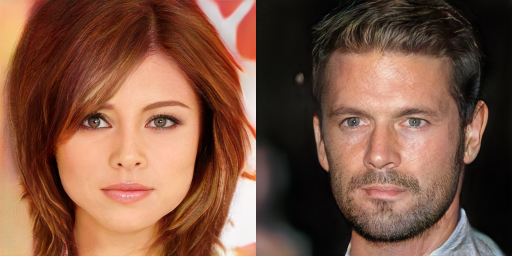
\includegraphics[width=0.8\textwidth]{figures/two_celebs}
        \end{figure}

        \begin{center}
            ``Two imaginary celebrities that were dreamed up by a random number generator.''
        \end{center}

        \source{https://research.nvidia.com/publication/2017-10\_Progressive-Growing-of}
    \end{frame}

    \begin{frame}{Why care about GANs?}
    Why to spend your limited time learning about GANs:
    \begin{itemize}
        \item GANs are achieving state-of-the-art results in a large variety of image generation tasks.
        \item There's been a veritable explosion in GAN publications over the last few years -- many people are very excited!
        \item GANs are stimulating new theoretical interest in min-max optimization problems and ``smooth games''.
    \end{itemize}

    \end{frame}

    \begin{frame}{Why care about GANs: Hyper-realistic Image Generation}

        \begin{center}
            StyleGAN: image generatation with hierarchical style transfer \cite{karras2018style}.
        \end{center}

        \begin{figure}
            \centering
            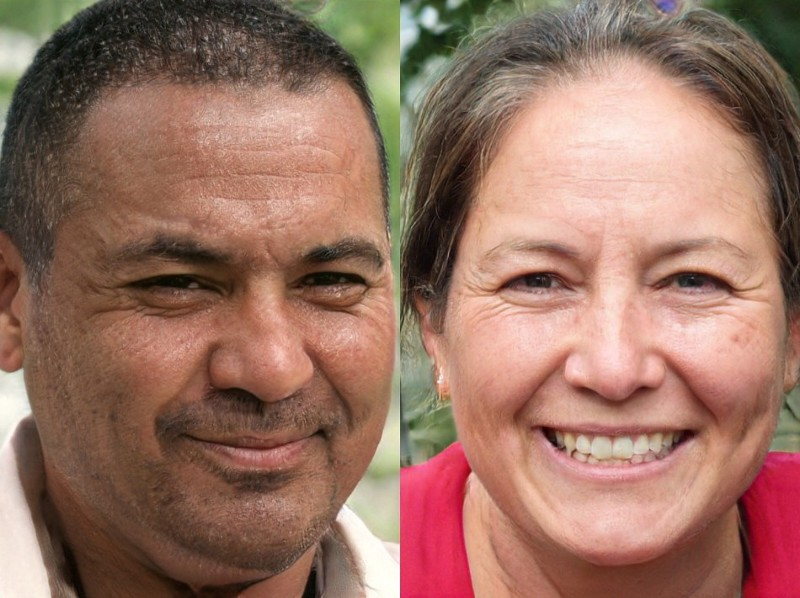
\includegraphics[width=0.7\textwidth]{figures/style_transfer}
        \end{figure}

        \source{https://arxiv.org/abs/1812.04948}
    \end{frame}


    \begin{frame}{Why care about GANs: Conditionally Generative Models}

        \begin{center} Conditional GANs: high-resolution image synthesis via semantic labeling \cite{wang2018high}. \end{center}

        \begin{center} \hspace{0.5cm} \textbf{Input: Segmentation} \hspace{0.5cm} \textbf{Output: Synthesized Image} \end{center}

        \begin{figure}
            \centering
            \begin{minipage}{.45\textwidth}
                \centering
                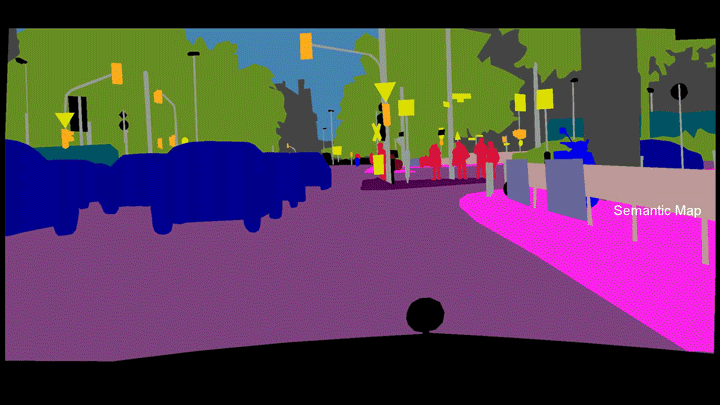
\includegraphics[width=1\textwidth]{figures/condit_gen/frame_00}
            \end{minipage}
            \begin{minipage}{.45\textwidth}
                \centering
                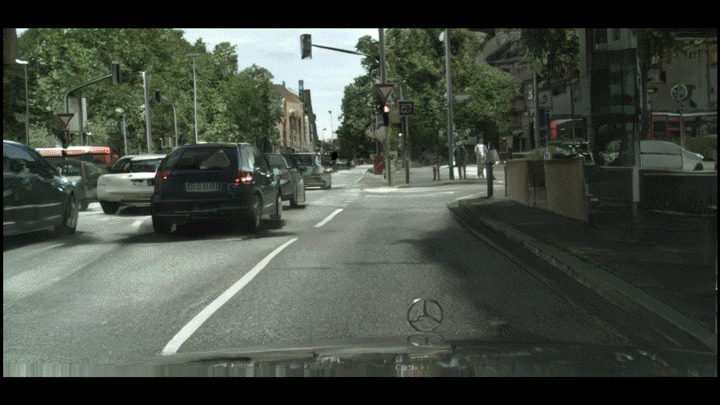
\includegraphics[width=1\textwidth]{figures/condit_gen/frame_58}
            \end{minipage}
        \end{figure}

        \source{https://research.nvidia.com/publication/2017-12\_High-Resolution-Image-Synthesis}

    \end{frame}

    \begin{frame}{Why care about GANs: Image Super Resolution}

        \begin{center} SRGAN: Photo-realistic super-resolution \cite{ledig2017photo}. \end{center}

        \begin{center} \textbf{Bicubic Interp.} \hspace{1.1cm} \textbf{SRGAN} \hspace{1.1cm} \textbf{Original Image} \end{center}
        \begin{figure}
            \centering
            \begin{minipage}{.3\textwidth}
                \centering
                
\includegraphics[width=1\textwidth]{figures/super_res/comic_SRF_4_bicubic}
            \end{minipage}
            \begin{minipage}{.3\textwidth}
                \centering
                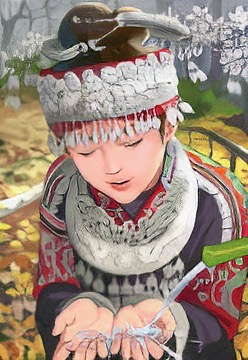
\includegraphics[width=1\textwidth]{figures/super_res/comic_SRGAN-VGG54}
            \end{minipage}
            \begin{minipage}{.3\textwidth}
                \centering
                
\includegraphics[width=1\textwidth]{figures/super_res/comic_HR}
            \end{minipage}
        \end{figure}

        \source{https://arxiv.org/abs/1609.04802}

    \end{frame}

    \begin{frame}{Why care about GANs: Publications}

        \begin{figure}
            \centering
            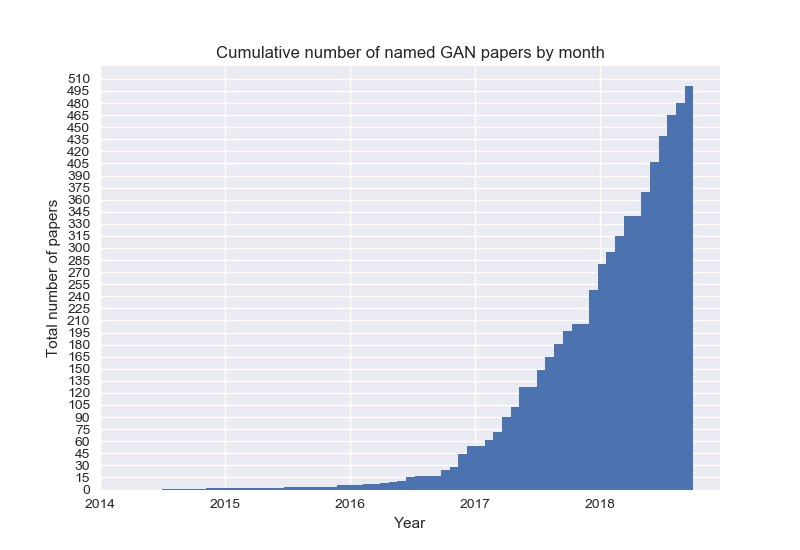
\includegraphics[width=0.8\textwidth]{figures/gan_papers}
        \end{figure}

        \begin{center} Approximately 500 papers GAN papers as of September 2018! \end{center}

        \source{See https://github.com/hindupuravinash/the-gan-zoo for the exhaustive list of papers.}
        \source{Image Credit: https://github.com/bgavran. }

    \end{frame}

    \section{Generative Models}

    \begin{frame}{Generative Modeling}
        \textbf{Generative Models} estimate the probabilistic process that generated a set of observations $\mathcal{D}$.
        \begin{itemize}
            \item $\mathcal{D} = \cbr{\rbr{\xx^i, \yy^i}}_{i=1}^n$: supervised generative models learn the joint distribution $p(\xx^i,\yy^i)$, often to compute $p(\yy^i \mid \xx^i)$.
            \item $\mathcal{D} = \cbr{\xx^i}_{i=1}^n$: unsupervised generative models learn the distribution of $\mathcal{D}$ for clustering, sampling, etc. We can:
            \begin{itemize}
                \item directly estimate $p(\xx^i)$,
                \item introducing latents $\yy^i$ and estimate $p(\xx^i, \yy^i)$.
            \end{itemize}
        \end{itemize}

    \end{frame}

    \begin{frame}{Generative Modeling: Unsupervised Parametric Approaches}

        \begin{itemize}
            \item \textbf{Direct Estimation:} Choose a parameterized family $p(\xx \mid \vtheta)$ and learn $\vtheta$ by maximizing the log-likelihood
            \begin{align*}
                \vtheta^{*} = \argmax{\vtheta} \sum_{i=1}^n \log p(\xx^i \mid \vtheta).
            \end{align*}
            \item \textbf{Latent Variable Models:} Define a joint distribution $p(\xx, \yy \mid \vtheta)$ and learn $\vtheta$ by maximizing the log-marginal likelihood
            \begin{align*}
                \vtheta^{*} = \argmax{\vtheta} \sum_{i=1}^n \log \int_{\zz^i} p(\xx^i, \zz^i \mid \vtheta) d \zz.
            \end{align*}
        \end{itemize}

        Both approaches require that $p(\xx \mid \vtheta)$ is easy to evaluate.
    \end{frame}

    \begin{frame}{Generative Modeling: Models for (Very) Complex Data}
        \begin{center} How can we learn such models for very complex data? \end{center}
            \vspace{0.2cm}

        \begin{figure}
            \centering
            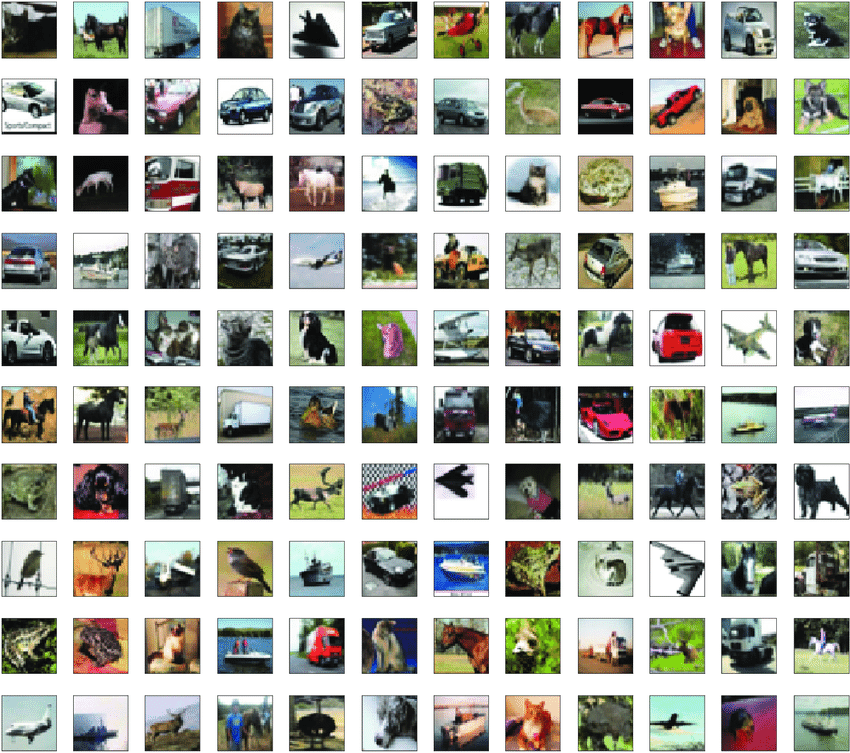
\includegraphics[width=0.6\textwidth]{figures/cifar}
        \end{figure}

        \source{https://www.researchgate.net/figure/Heterogeneousness-and-diversity-of-the-CIFAR-10-entries-in-their-10-image-categories-The\_fig1\_322148855}

    \end{frame}

    \begin{frame}{Generative Modeling: Normalizing Flows and VAEs}

        Design parameterized densities with huge capacity!

        \begin{itemize}
            \item \textbf{Normalizing flows:} sequence of non-linear transformations to a simple distribution $p_{\zz}(\zz)$
            \[ p(\xx \mid \vtheta_{0:k}) = p_{\zz}(\zz) \ \text{where} \ \zz = f^{-1}_{\vtheta_k} \circ \dots \circ f^{-1}_{\vtheta_1} \circ f^{-1}_{\vtheta_0} \rbr{\xx}. \]
            $f^{-1}_{\theta_j}$ must be invertible with tractable log-det. Jacobians.
            \item \textbf{VAEs:} latent-variable models where inference networks specify parameters
            \[ p(\xx, \yy \mid \vtheta ) = p(\xx \mid f_\vtheta(\yy)) p_{\yy}(\yy). \]
            The marginal likelihood is maximized via the ELBO.
        \end{itemize}
    \end{frame}

    \section{GANs}

    \begin{frame}{GANs: Density-Free Models}
        \textbf{Generative Adversial Networks (GANs)} instead use an unrestricted generator $G_{\vtheta_g}(\zz)$ such that
        \[ p(\xx \mid \vtheta_g) = p_{\zz}(\cbr{\zz}) \ \text{where} \ \cbr{\zz} = G_{\vtheta_g}^{-1}(\xx). \]
        \vspace{-0.75cm}
        \begin{itemize}
            \item \textbf{Problem:} the inverse image of $G_{\vtheta_g}(\zz)$ may be huge!
            \item \textbf{Problem:} it's likely intractable to preserve volume through $G(\zz; \vtheta_g)$.
        \end{itemize}
        So, we can't evaluate $p(\xx \mid \vtheta_g)$ and we can't learn $\vtheta_g$ by maximum likelihood.

    \end{frame}

    \begin{frame}{GANs: Discriminators}
        GANs learn by comparing model samples with examples from $\mathcal{D}$.
        \begin{itemize}
            \item Sampling from the generator is easy:
            \[ \hat \xx = G_{\vtheta_g}(\hat \zz), \ \text{where} \ \hat \zz \sim p_{\zz}(\zz). \]
            \item Given a sample $\hat \xx$, a discriminator tries to distinguish it from true examples:
            \[ D(\xx) = \text{Pr}\rbr{\xx \sim p_{\text{data}} }. \]
            \item The discriminator ``supervises'' the generator network.
        \end{itemize}

    \end{frame}

    \begin{frame}{GANs: Generator + Descriminator}

        \begin{figure}
            \centering
            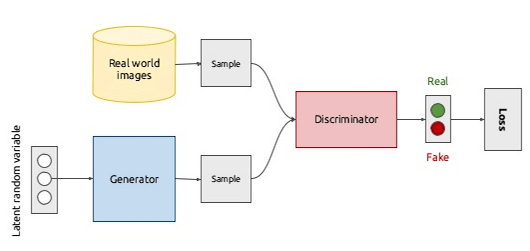
\includegraphics[width=0.95\textwidth]{figures/gan_conceptual}
        \end{figure}

        \source{https://www.slideshare.net/xavigiro/deep-learning-for-computer-vision-generative-models-and-adversarial-training-upc-2016}

    \end{frame}

    \begin{frame}{GANs: Goodfellow et al. (2014)}

        \begin{itemize}
            \item Let $\zz \in \R^{m}$ and $p_{\zz}(\zz)$ be a simple base distribution.
            \item The generator $G_{\vtheta_g}(\zz): \R^m \rightarrow \mathcal{\tilde D}$ is a deep neural network.
            \begin{itemize}
                \item $\mathcal{\tilde D}$ is the manifold of generated examples.
            \end{itemize}
            \item The discriminator $D_{\vtheta_d}(\xx): \mathcal{D} \cup \mathcal{\tilde D} \rightarrow \rbr{0,1}$ is also a deep neural network.
        \end{itemize}
        \vspace{0.4cm}

        \begin{figure}
            \centering
            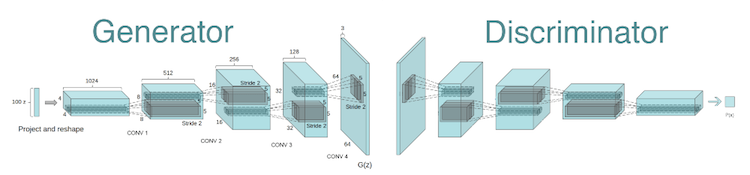
\includegraphics[width=0.98\textwidth]{figures/conv_gan}
        \end{figure}

        \source{https://arxiv.org/abs/1511.06434}

    \end{frame}

    \begin{frame}{GANs: Saddle-Point Optimization}
        \textbf{Saddle-Point Optimization:} learn $G_{\vtheta_g}(\zz)$ and $D_{\vtheta_d}(\xx)$ jointly via the objective $V(\vtheta_d, \vtheta_g)$:
        \[ \min_{\vtheta_g} \max_{\vtheta_d} \ \underbrace{\E_{p_{\text{data}}} \sbr{\log D_{\vtheta_d}(\xx)}}_{\text{likelihood of true data}} + \underbrace{\E_{p_{\zz}(\zz)} \sbr{\log \rbr{1 - D_{\vtheta_d}(G_{\vtheta_g}(\zz))}}}_{\text{likelihood of generated data}} \]
        \vspace{-1cm}
        \begin{figure}
            \centering
            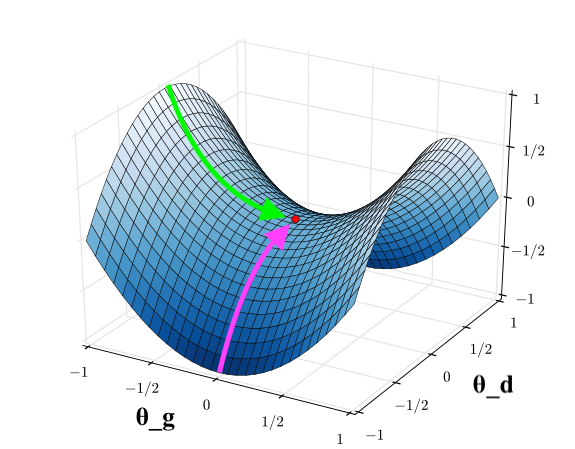
\includegraphics[width=0.75\textwidth]{figures/saddle_point_drawing}
        \end{figure}
    \end{frame}

    \begin{frame}{GANs: Optimal Discriminators}

        \textbf{Claim:} Given $G_{\vtheta_g}$ defining an implicit distribution $p_g = p(\xx \mid \vtheta_g)$,
        the optimal descriminator is
        \[ D^*(\xx) = \frac{p_{\text{data}}(\xx)}{p_{\text{data}}(\xx) + p_{\text{g}}(\xx)}. \]
        \textbf{Proof Sketch:}
        \begin{align*}
            V(\vtheta_d, \vtheta_g) &= \int_{\mathcal{D}} p_{\text{data}}(\xx) \log D(\xx) d \xx + \int_{\mathcal{\tilde D}} p(\zz)\log(1-D(G_{\theta_g}(\zz))) d \zz\\
            &= \int_{\mathcal{D} \cup \mathcal{\tilde D}} p_{\text{data}}(\xx) \log D(\xx) + p_g(\xx)\log(1-D(\xx)) d \xx
        \end{align*}
        Maximizing the integrand for all $\xx$ is sufficient and gives the result (see bonus slides).
        \source{Previous Slide: https://commons.wikimedia.org/wiki/File:Saddle\_point.svg}
    \end{frame}

    \begin{frame}{GANs: Jensen-Shannon Divergence and Optimal Generators}
        Given an optimal discriminator $D^*(\xx)$, the generator objective is
        \begin{align*}
            C(\vtheta_g) &= \E_{p_{\text{data}}} \sbr{\log D^*_{\vtheta_d}(\xx)} + \E_{p_g(\xx)} \sbr{\log \rbr{1 - D^*_{\vtheta_d}(\xx)}}\\ \\
            &= \E_{p_{\text{data}}} \sbr{\log \frac{p_{\text{data}}(\xx)}{p_{\text{data}}(\xx) + p_{\text{g}}(\xx)}} + \E_{p_{g}(\xx)} \sbr{\log \frac{p_{g}(\xx)}{p_{\text{data}}(\xx) + p_{\text{g}}(\xx)}}\\ \\
            &\propto \underbrace{\half KL\rbr{p_{\text{data}} \biggmid \biggmid \frac{\rbr{p_{\text{data}} + p_g}}{2}} + \half KL\rbr{p_{g} \biggmid \biggmid \frac{\rbr{p_{\text{data}} + p_g}}{2}}}_{\text{Jensen-Shannon Divergence}}
        \end{align*}
        $C(\vtheta_g)$ achives its global minimum at $p_g = p_{\text{data}}$ given an optimal discriminator!
    \end{frame}

    \begin{frame}{GANs: Learning Generators and Discriminators}
        Putting these results to use in practice:
        \begin{itemize}
            \item High-capacity discriminators $D_{\vtheta_d}$ approximate the Jensen-Shannon divergence when close to global maximum.
            \item $D_{\vtheta_d}$ is a ``differentiable program''.
            \item We can use $D_{\vtheta_d}$ to learn $G_{\vtheta_g}$ with our favourite gradient descent method.
        \end{itemize}

        \begin{figure}
            \centering
            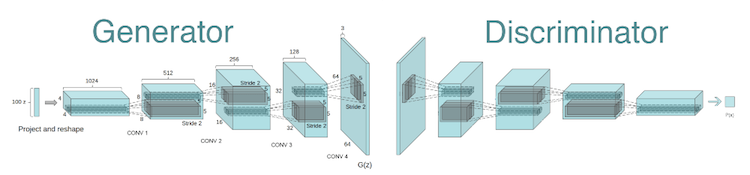
\includegraphics[width=0.98\textwidth]{figures/conv_gan}
        \end{figure}

        \source{https://arxiv.org/abs/1511.06434}

    \end{frame}

    \begin{frame}{GANs: Training Procedure}
        \vspace{-0.4cm}
        \begin{center} \rule{10.5cm}{0.05cm} \end{center}
        \begin{algorithmic}
            \FOR{$i = 1 \dots N$}
              \FOR{$k = 1 \dots K$}
                \STATE{$\bullet$ Sample noise samples $\{ \zz^{1}, \dots, \zz^{m} \} \sim p_{\zz}(\zz)$}
                \STATE{$\bullet$ Sample examples $\{ \xx^{1}, \dots, \xx^{m} \}$ from $p_\text{data}(\xx)$.}
                \STATE{$\bullet$ Update the discriminator $D_{\vtheta_d}$:
                    \[
                        \theta_d = \theta_d - \alpha_d \nabla_{\theta_d} \frac{1}{m} \sum_{i=1}^m \left[
                        \log D\left(\xx^{i}\right)
                        + \log \left(1-D\left(G\left(\zz^{i}\right)\right)\right)
                        \right].
                    \]}
               \ENDFOR
              \STATE{$\bullet$ Sample noise samples $\{ \zz^{1}, \dots, \zz^{m} \} \sim p_{\zz}(\zz)$.}
                \STATE{$\bullet$ Update the generator $G_{\vtheta_g}$:
                    \[
                        \theta_g = \theta_g - \alpha_g \nabla_{\theta_g} \frac{1}{m} \sum_{i=1}^m
                        \log \left(1-D\left(G\left(\zz^{i}\right)\right)\right).
                    \]}
              \ENDFOR
        \end{algorithmic}
        \vspace{-0.5cm}
        \begin{center} \rule{10.5cm}{0.05cm} \end{center}

    \end{frame}

    \section{Problems (c. 2016)}

    \begin{frame}{Problems with GANs}

        \begin{itemize}
            \item \textbf{Vanishing gradients:} the discriminator becomes "too good" and the generator gradient vanishes.
            \item \textbf{Non-Convergence:} the generator and discriminator oscillate without reaching an equilibrium.
            \item \textbf{Mode Collapse:} the generator distribution collapses to a small set of examples.
            \item \textbf{Mode Dropping:} the generator distribution doesn't fully cover the data distribution.
        \end{itemize}

    \end{frame}


    \begin{frame}{Problems: Vanishing Gradients}

        \begin{itemize}
            \item The \textbf{minimax} objective saturates when $D_{\vtheta_d}$ is close to perfect:
            \[ V(\vtheta_d, \vtheta_g) = \E_{p_{\text{data}}} \sbr{\log D_{\vtheta_d}(\xx)} + \E_{p_{\zz}(\zz)} \sbr{\log \rbr{1 - D_{\vtheta_d}(G_{\vtheta_g}(\zz))}}. \]
            \item A \textbf{non-saturating heuristic} objective for the generator is
            \[ J(G_{\vtheta_g}) = - \E_{p_{\zz}(\zz)} \sbr{\log \rbr{D_{\vtheta_d}(G_{\vtheta_g}(\zz))}}. \]
        \end{itemize}

        \begin{figure}
            \centering
            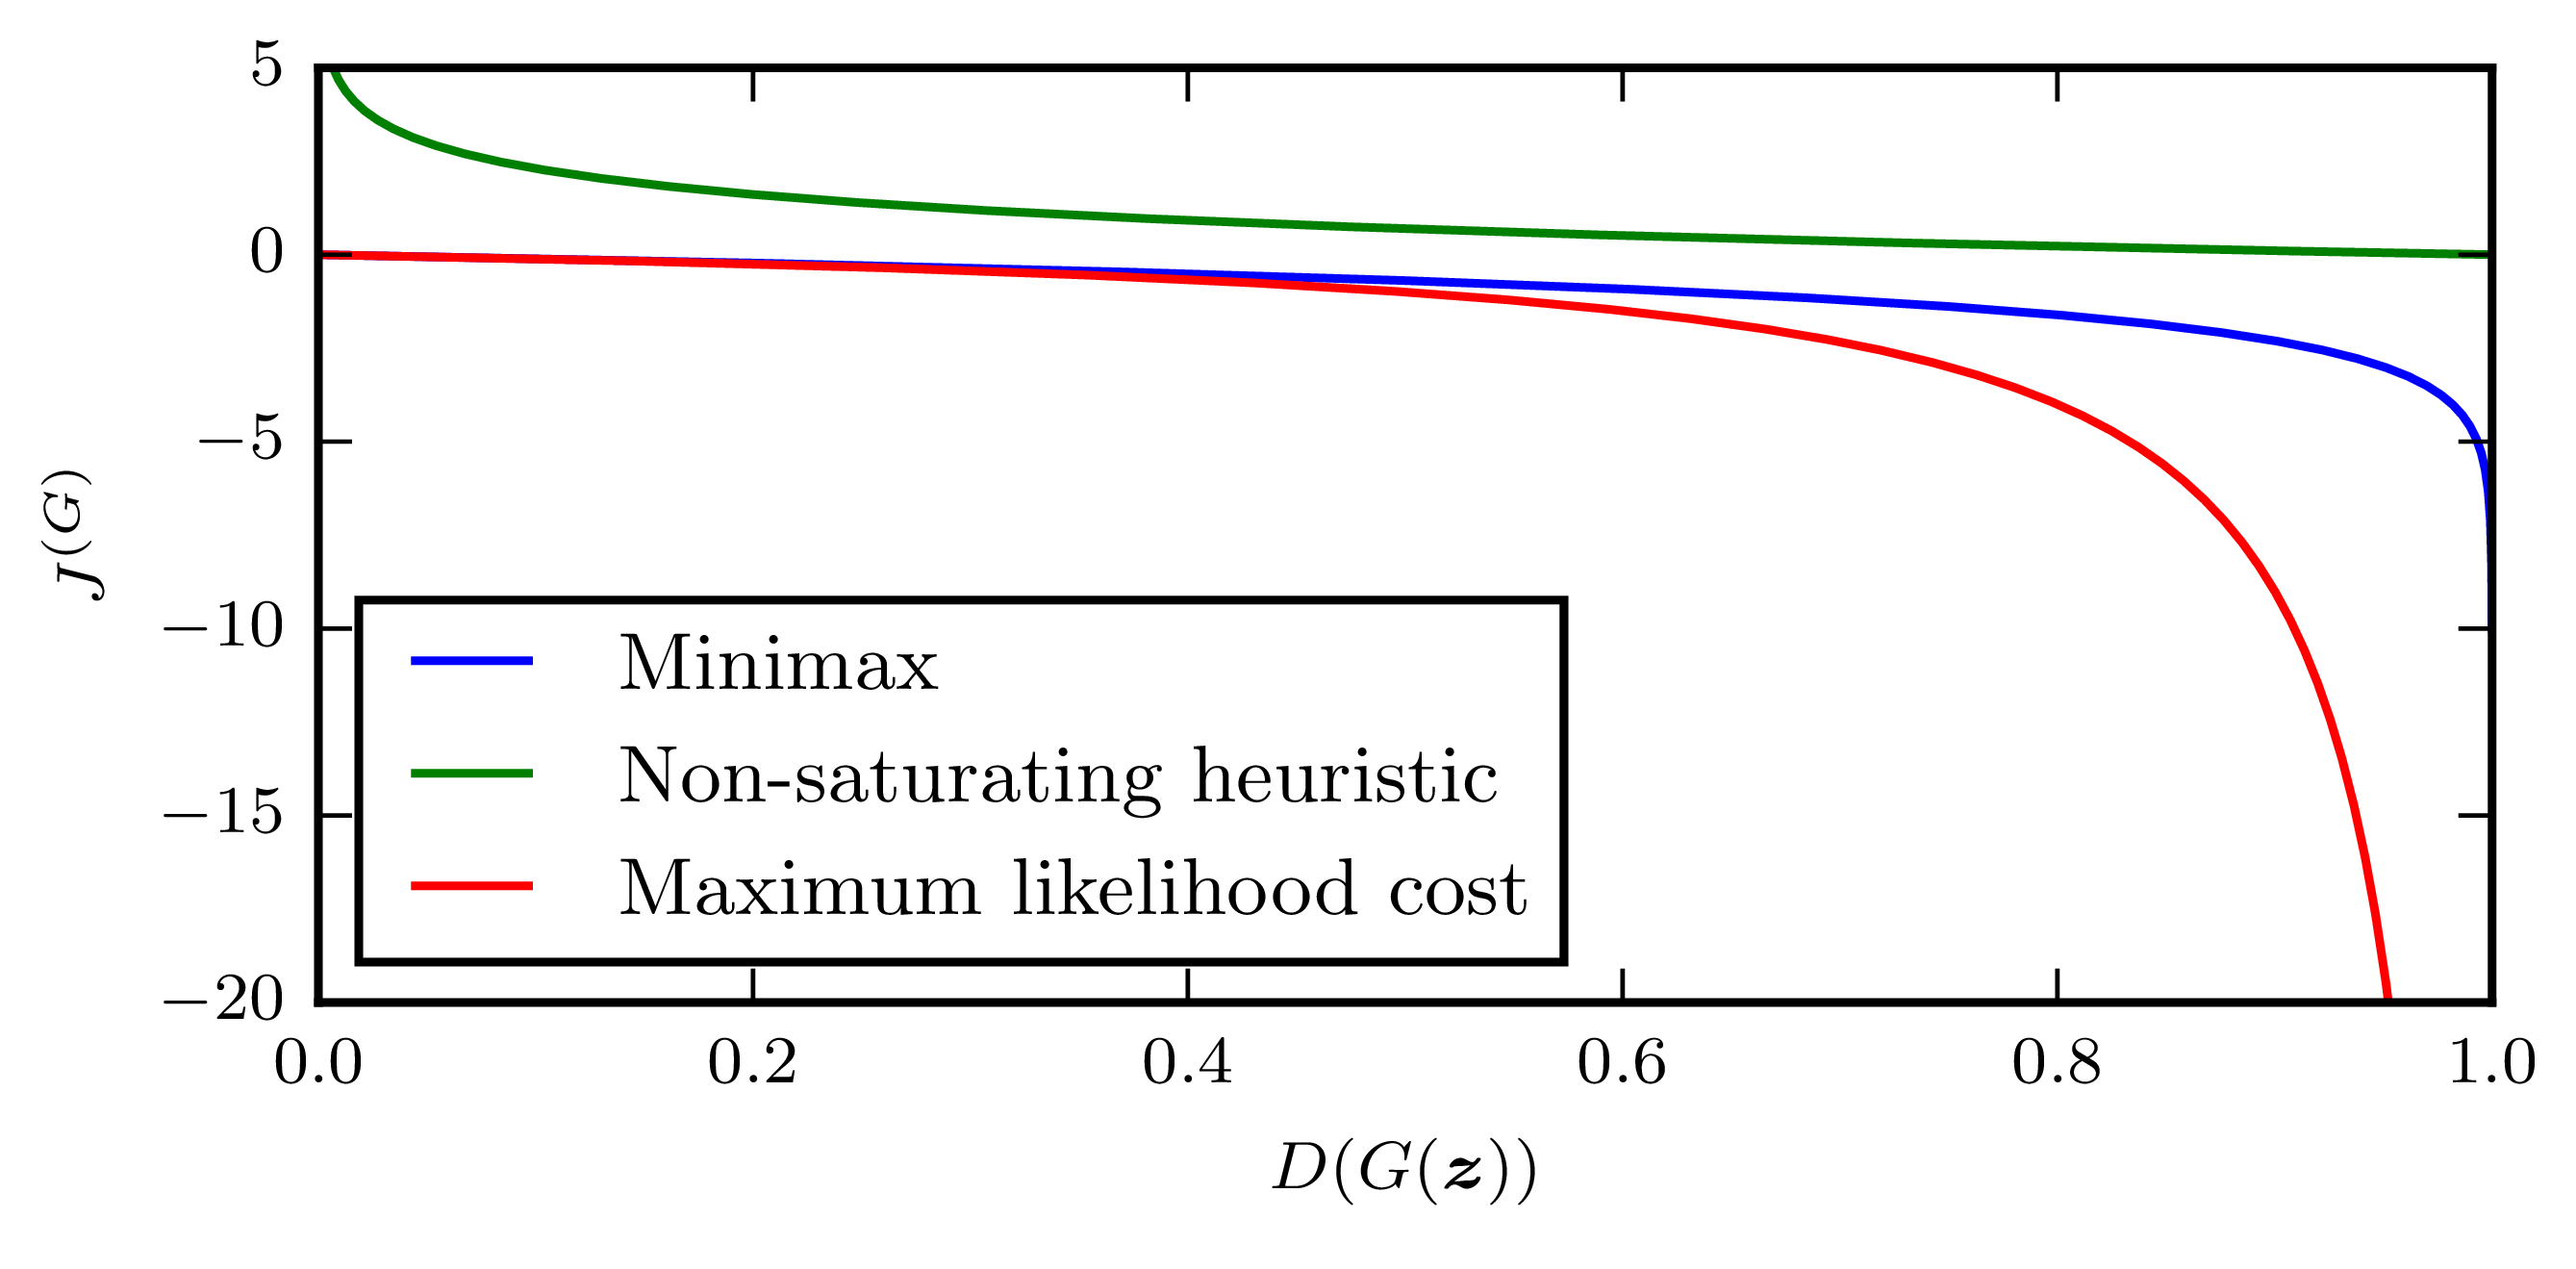
\includegraphics[width=0.8\textwidth]{figures/vanish}
        \end{figure}
        \vspace{-0.5cm}
        \source{https://arxiv.org/abs/1701.00160}

    \end{frame}

    \begin{frame}{Problems: Addressing Vanishing Gradients}
        \textbf{Solutions: }
        \begin{itemize}
            \item \textbf{Change Objectives:} use the non-saturating heuristic objective, maximum-likelihood cost, etc.
            \item \textbf{Limit Discriminator:} restrict the capacity of the discriminator.
            \item \textbf{Schedule Learning:} try to balance training $D_{\vtheta_d}$ and $G_{\vtheta_g}$.
        \end{itemize}

    \end{frame}

    \begin{frame}{Problems: Non-Convergence}

        Simultaneous gradient descent is not guaranteed to converge for minimax objectives.
        \begin{itemize}
            \item Goodfellow et al. only showed convergence when updates are made in the function space \cite{goodfellow2014generative}.
            \item The parameterization of $D_{\vtheta_d}$ and $G_{\vtheta_g}$ results in highly non-convex objective.
            \item In practice, training tends to oscillate -- updates ``undo'' each other.
        \end{itemize}
    \end{frame}

    \begin{frame}{Problems: Addressing Non-Convergence}

        \textbf{Solutions: } Lots and lots of hacks!

        \begin{figure}
            \centering
            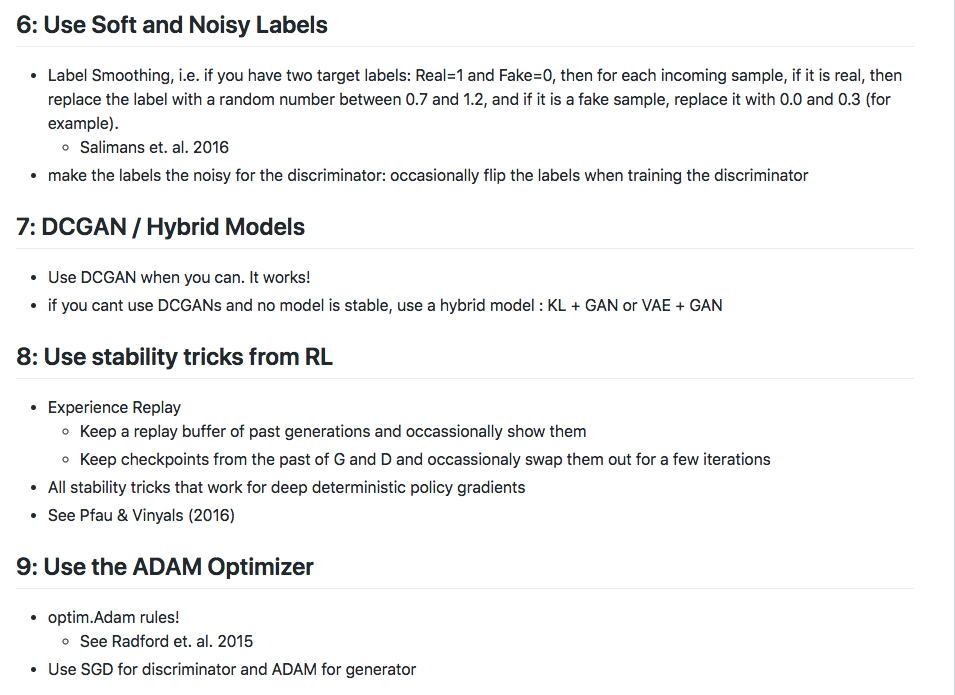
\includegraphics[width=0.8\textwidth]{figures/hacks}
        \end{figure}

        \source{https://github.com/soumith/ganhacks}

    \end{frame}

    \begin{frame}{Problems: Mode Collapse and Mode Dropping}
        \textbf{One Explanation:} SGD may optimize the max-min objective
        \[ \max_{\vtheta_d} \min_{\vtheta_g} \E_{p_{\text{data}}} \sbr{\log D_{\vtheta_d}(\xx)} + \E_{p_{\zz}(\zz)} \sbr{\log \rbr{1 - D_{\vtheta_d}(G_{\vtheta_g}(\zz))}} \]
        \textbf{Intuition:} the generator maps all $\zz$ values to the $\hat \xx$ that is mostly likely to fool the discriminator.
        \source{https://arxiv.org/abs/1701.00160}

        \begin{figure}
            \centering
            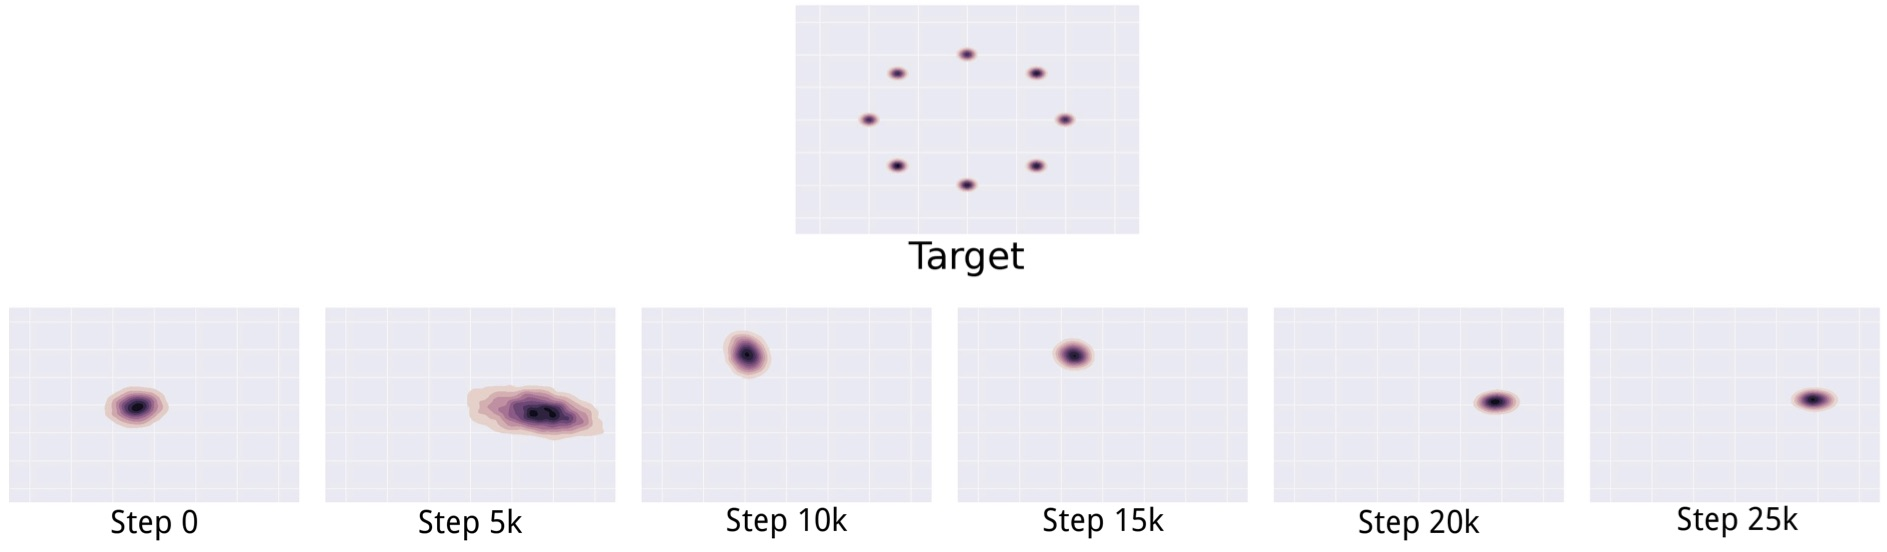
\includegraphics[width=0.98\textwidth]{figures/mode_collapse}
        \end{figure}

    \end{frame}

    \section{A Possible Solution}

    \begin{frame}{A Possible Solution: Alternative Divergences}
        There are a large variety of divergence measures for distributions:
        \begin{itemize}
            \item \textbf{f-Divergences:} (e.g. Jensen-Shannon, Kullback-Leibler)
            \[ D_f \ (P \ || Q) = \int_{\chi} q(\xx) f(\frac{p(\xx)}{q(\xx)}) d\xx \]
            \begin{itemize}
                \item GANs \cite{goodfellow2014generative}, f-GANs \cite{nowozin2016f}, and more.
            \end{itemize}
            \item \textbf{Integral Probability Metrics:} (e.g. Earth Movers Distance, Maximum Mean Discrepancy)
            \[ \gamma_{F} \ (P \ || Q) = \sup_{f \in F} \biggmid \int f dP - \int f dQ \ \biggmid \]
            \begin{itemize}
                \item Wasserstein GANs \cite{arjovsky2017wasserstein}, Fisher GANs \cite{mroueh2017fisher}, Sobolev GANs \cite{mroueh2017sobolev} and more.
            \end{itemize}
        \end{itemize}
    \end{frame}

    \begin{frame}{A Possible Solution: Wasserstein GANs}

        \textbf{Wasserstein GANs:} Strong theory and excellent empirical results.
        \vspace{-0.6cm}
        \begin{itemize}
            \item ``In no experiment did we see evidence of mode collapse for the WGAN algorithm.'' \cite{arjovsky2017wasserstein}
        \end{itemize}
        \vspace{-0.2cm}
        \begin{figure}
            \centering
            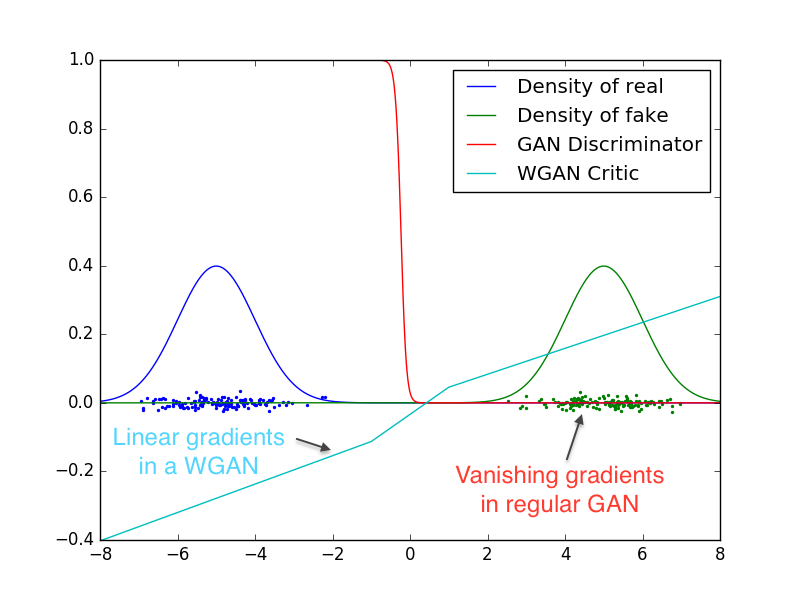
\includegraphics[width=0.7\textwidth]{figures/wasserstein}
        \end{figure}
        \vspace{-0.5cm}
        \source{https://arxiv.org/abs/1701.07875}

    \end{frame}

    \section{Summary}

    \begin{frame}{Summary}

        \textbf{Recap:}
        \begin{itemize}
            \item GANs are a class of density-free generative models with (mostly) unrestricted generator functions.
            \item Introducing adversial discriminator networks allows GANs to learn by minimizing the Jensen-Shannon divergence.
            \item Concurrently learning the generator and discriminator is challenging due to
                \begin{itemize}
                    \item Vanishing Gradients,
                    \item Non-convergence due to oscilliation
                    \item Mode collapse and mode dropping.
                \end{itemize}
            \item A variety of alternative objective functions are being proposed.
        \end{itemize}

    \end{frame}

    \begin{frame}{Agknowledgements and References}

        There are lots of excellent references on GANs:
        \begin{itemize}
            \item Sebastian Nowozin's {\color{blue} \href{https://github.com/nowozin/mlss2018-madrid-gan}{presentation}} at MLSS 2018.
            \item NIPS 2016 {\color{blue} \href{https://arxiv.org/abs/1701.00160}{tutorial}} on GANs by Ian Goodfellow.
            \item A {\color{blue} \href{https://www.alexirpan.com/2017/02/22/wasserstein-gan.html}{nice explanation}} of Wasserstein GANs by Alex Irpan.
        \end{itemize}

    \end{frame}

    \begin{frame}{Bonus: Optimal Discriminators Cont.}
        The integrand
        \[ h(D(\xx)) = p_{\text{data}}(\xx) \log D(\xx) + p_g(\xx)\log(1-D(\xx)) \]
        is concave for $D(\xx) \in (0,1)$. We take the derivative and compute a stationary point in the domain:
        \begin{align*}
            \frac{\partial h(D(\xx))}{\partial D(\xx)} &= \frac{p_{\text{data}}(\xx)}{D(\xx)} - \frac{p_g(\xx)}{1-D(\xx)} = 0\\
            \Rightarrow D(\xx) &= \frac{p_{\text{data}}(\xx)}{p_{\text{data}}(\xx) + p_{\text{g}}(\xx)}.
        \end{align*}
        This minimizes the integrand over the domain of the discriminator, completing the proof.
    \end{frame}

    \begin{frame}[allowframebreaks]{References}
        \bibliographystyle{plain}
        \bibliography{refs}
    \end{frame}

\end{document}
